\chapter{Cơ sở lý thuyết} \label{sec:chuong-2}

\section{Lý thuyết về xử lý ảnh:}
	
	\subsection{Mạng Neuron tích chập (CNN):}
	\subsubsection{Tích chập (Convolution)}
	Trong xử lý số tín hiệu , tích chập là một khái niệm hết sức quen thuộc, nó là một phép toán cho 2 hàm số để ra một hàm số khác phép tích chập có thể thể hiện nhiều kiểu biến đổi (có thể là lọc tín hiệu, xét xem tín hiệu có theo mẫu nào không,....) 
	
		\begin{figure} [h!]
		\begin{center}
			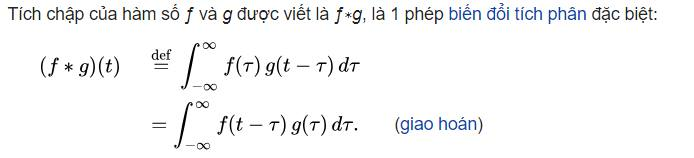
\includegraphics[width=0.75\textwidth,keepaspectratio]
			{tichchap_ct.png}
		\end{center}
		\caption{Công thức tích chập} 
		\label{fig:pho-ofdm} 
	\end{figure}

    Công thức của tích chập thể hiện tính chất của tích chập đó là khi thực hiện, ta phải trừ ngược lại đáp ứng xung của hệ thống để tích chập thực hiện trước khi tín hiệu xuất hiện (thể hiện việc tín hiệu có thể xuất hiện ở trước điểm 0)
	
	Trong đó ta thực hiện trừ ngược và lật hàm g lại sau đó tích phân trên cả miền của tín hiệu
		\begin{figure} [h!]
		\begin{center}
			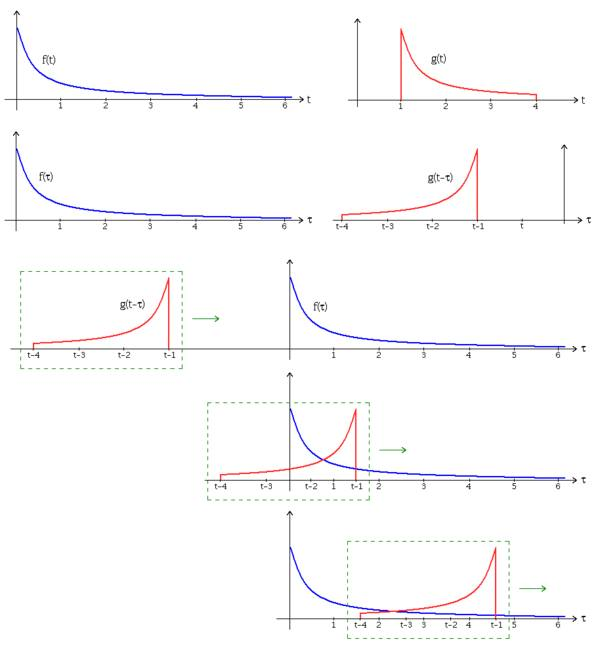
\includegraphics[width=0.75\textwidth,keepaspectratio]
			{tichchap.png}
		\end{center}
		\caption{Biểu diễn tích chập} 
		\label{fig:pho-ofdm} 
	\end{figure}


Ta hoàn toàn có thể coi đây như là tín hiệu 2 chiều vậy, chính vì vậy để lọc các tính chất của ảnh ta có thể áp dụng được các công cụ như tích chập. Chính vì thế dẫn đến các bộ lọc được dùng rất nhiều trong computer vision. Tuy nhiên ở đây tín hiệu có 2 chiều, và hơn nữa lại không có trường hợp tín hiệu xuất hiện trước t = 0 nên tích chập ở đây không cần phải lật kernel như tín hiệu 1 chiều. Chính vì vậy nó giống một khái niệm khác là tương quan chéo, mặc dù bản chất không giống nhau, phép này vẫn là tích chập.

Công thức của tích chập 2 chiều:

\begin{figure} [h!]
	\begin{center}
		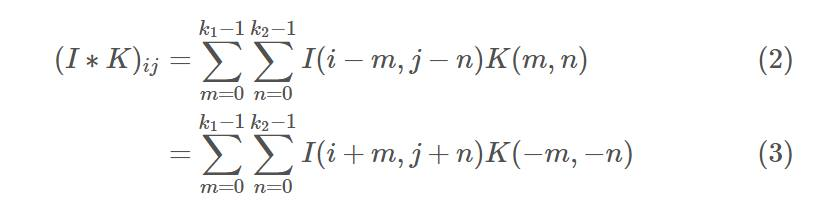
\includegraphics[width=0.5\textwidth,keepaspectratio]
		{matconv.png}
	\end{center}
	\caption{Biểu diễn tích chập} 
	\label{fig:pho-ofdm} 
\end{figure}


Ở đây có thể thấy phép convolution được thực hiện giống với 1 chiều, và phép tích phân được thay thế bằng phép tổng, phù hợp với tín hiệu rời rạc






	\subsubsection{Mạng neuron tích chập}
	
	
	Mạng Nơ-ron Tích Chập có kiến trúc khác với Mạng Nơ-ron thông thường. Mạng Nơ-ron bình thường chuyển đổi đầu vào thông qua hàng loạt các tầng ẩn. Mỗi tầng là một tập các nơ-ron và các tầng được liên kết đầy đủ với các nơ-ron ở tầng trước đó. Và ở tầng cuối cùng sẽ là tầng kết quả đại diện cho dự đoán của mạng.
	
	Đầu tiên, mạng Nơ-ron Tích Chập được chia thành 3 chiều: rộng, cao, và sâu. Kế đên, các nơ ron trong mạng không liên kết hoàn toàn với toàn bộ nơ-ron kế đến nhưng chỉ liên kết tới một vùng nhỏ. Cuối cùng, một tầng đầu ra được tối giản thành véc-tơ của giá trị xác suất.
	
	CNNs gồm hai thành phần:
		\begin{figure} [h!]
		\begin{center}
			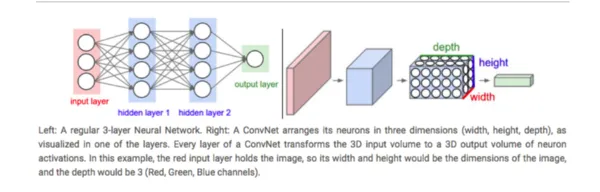
\includegraphics[width=0.75\textwidth,keepaspectratio]
			{cnn_1.png}
		\end{center}
		\caption{Biểu diễn tích chập} 
		\label{fig:pho-ofdm} 
	\end{figure}


	•	Phần tầng ẩn hay phần rút trích đặc trưng: trong phần này, mạng sẽ tiến hành tính toán hàng loạt phép tích chập và phép hợp nhất (pooling) để phát hiện các đặc trưng. Ví dụ: nếu ta có hình ảnh con ngựa vằn, thì trong phần này mạng sẽ nhận diện các sọc vằn, hai tai, và bốn chân của nó.
	
	
	•	Phần phân lớp: tại phần này, một lớp với các liên kết đầy đủ sẽ đóng vai trò như một bộ phân lớp các đặc trưng đã rút trích được trước đó. Tầng này sẽ đưa ra xác suất của một đối tượng trong hình.
	
	
	
	Tích chập là một khối quan trọng trong CNN. Thuật ngữ tích chập được dựa trên một phép hợp nhất toán học của hai hàm tạo thành hàm thứ ba. Phép toán này kết hợp hai tập thông tin khác nhau.
	Trong trường hợp CNN, tích chập được thực hiện trên giá trị đầu vào của dữ liệu và kernel/filter (thuật ngữ này được sử dụng khác nhau tùy tình huống) để tạo ra một bản đồ đặc trưng (feature map).
	
	
	Ta thực hiện phép tích chập bằng cách trượt kernel/filter theo dữ liệu đầu vào. Tại mỗi vị trí, ta tiến hành phép nhân ma trận và tính tổng các giá trị để đưa vào bản đồ đặc trưng.
	
	
	Trong hình dưới đây, thành phần kernel/filter (màu xanh lá) trượt trên đầu vào (màu xanh dương) và kết quả được trả về bản đồ đặc trưng (màu đỏ). Kernel/filter có kích thước là 3×3 trong ví dụ này.
	
	
	Trong thực tế, tích chập được thực hiện hiện trên không gian 3 chiều. Vì mỗi hình ảnh được biểu diễn dưới dạng 3 chiều: rộng, cao, và sâu. Chiều sâu ở đây chính là giá trị màu sắc của hình (RGB).
	Ta thực hiện phép tích chập trên đầu vào nhiều lần khác nhau. Mỗi lần sử dụng một kernel/filter khác nhau. Kết quả ta sẽ thu được những bản đồ đặc trưng khác nhau. Cuối cùng, ta kết hợp toàn bộ bản đồ đặc trưng này thành kết quả cuối cùng của tầng tích chập.
	
	Tương tự như mạng nơ-ron thông thường, ta sử dụng một hàm kích hoạt (activate function) để có đầu ra dưới dạng phi tuyến. Trong trường hợp CNN, đầu ra của phép tích chập sẽ đi qua hàm kích hoạt nào đó ví dụ như hàm ReLU (rectified linear units).
	
	Trong quá trình trượt kernel/filter trên dữ liệu đầu vào, ta sẽ quy định một bước nhảy (stride) với mỗi lần di chuyển. Thông thường ta lựa chọn thường chọn bước nhảy là 1. Nếu kích thước bước nhảy tăng, kernel/filter sẽ có ít ô trùng lắp.
	
	Bởi vì kích thước đầu ra luôn nhỏ hơn đầu vào nên ta cần một phép xử lí đầu vào để đầu ra không bị co giãn. Đơn giản ta chỉ cần thêm một lề nhỏ vào đầu vào. Một lề với giá trị 0 sẽ được thêm vào xung quanh đầu vào trước khi thực hiện phép tích chập.
	
	Thông thường, sau mỗi tầng tích chập, ta sẽ cho kết quả đi qua một tầng hợp nhất (pooling layer). Mục đích của tầng này là để nhanh chóng giảm số chiều. Việc này giúp giảm thời gian học và hạn chế việc overfitting.
	
	Một phép hợp nhất đơn giản thường được dùng đó là max pooling, phép này lấy giá trị lớn nhất của một vùng để đại diện cho vùng đó. Kích thước của vùng sẽ được xác định trước để giảm kích thước của bản đồ đặc trưng nhanh chóng nhưng vẫn giữ được thông tin cần thiết.
	
	
	Tổng kết lại khi sử dụng CNN, ta cần chú ý đến 4 tham số quan trọng:
	•	Kích thước kernel/filter
	
	•	Số lượng kernel/filter
	
	•	Kích thước bước nhảy (stride)
	
	•	Kích thước lề (padding)
	
	\subsubsection{Phân lớp}
	
	
	Trong phần phân lớp, ta sử dụng một vài tầng với kết nối đầy đủ để xử lí kết quả của phần tích chập. Vì đầu vào của mạng liên kết đầy đủ là 1 chiều, ta cần làm phẳng đầu vào trước khi phân lớp. Tầng cuối cùng trong mạng CNN là một tầng liên kết đầy đủ, phần này hoạt động tương tự như mạng nơ-ron thông thường.
	
		\begin{figure} [h!]
		\begin{center}
			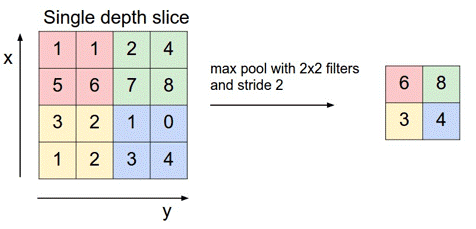
\includegraphics[width=0.75\textwidth,keepaspectratio]
			{cnn_3.png}
		\end{center}
		\caption{Biểu diễn tích chập} 
		\label{fig:pho-ofdm} 
	\end{figure}
	Kết quả thu được cuối cùng cũng sẽ là một véc-tơ với các giá trị xác suất cho việc dự đoán như mạng nơ-ron thông thường.
	
	
	
	Cài đặt Latex bao gồm hai phần là tập lệnh chính (Miktex) có trang chủ tại đây: \url{https://miktex.org/} và phần mềm giao diện với người dùng.
	Phần mềm giao diện có rất nhiều, tác giả báo cáo mẫu này dùng TexStudio (\url{http://www.texstudio.org/}) do là phần mềm miễn phí. 
\section{Long sort term memory}
\subsection{Recurrent Neural Network}
	Để thực hiện xử lý các giá trị có tính chất chuỗi (sequence) với mạng nơ-ron, kiến trúc Recurrent Neural Network được sử dụng. Mô hình này có cấu trúc như hình dưới:
	\begin{figure} [h!]
		\begin{center}
			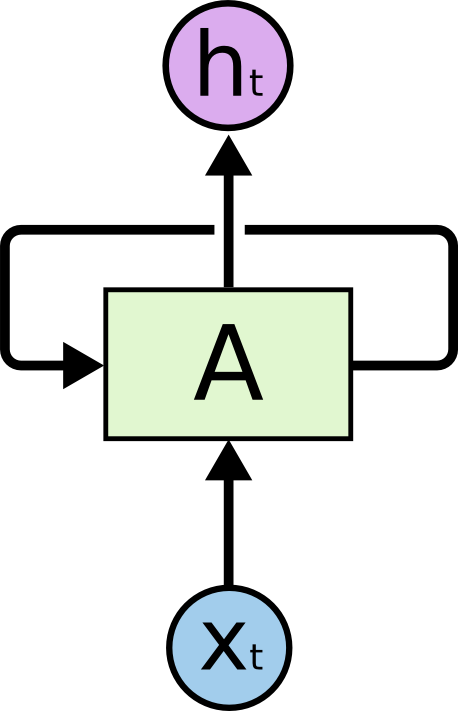
\includegraphics[width=0.25\textwidth,keepaspectratio]
			{RNN-rolled.png}
		\end{center}
		\caption{RNN unrolled} 
		\label{fig:pho-ofdm} 
	\end{figure}

    Hình trên là biểu diễn ý tưởng cơ bản của mạng nơ-ron RNN: dữ liệu từ các thời điểm khác nhau trong thời gian đều có ảnh hưởng đến dữ liệu ở thời điểm tiếp sau:

	\begin{figure} [h!]
	\begin{center}
		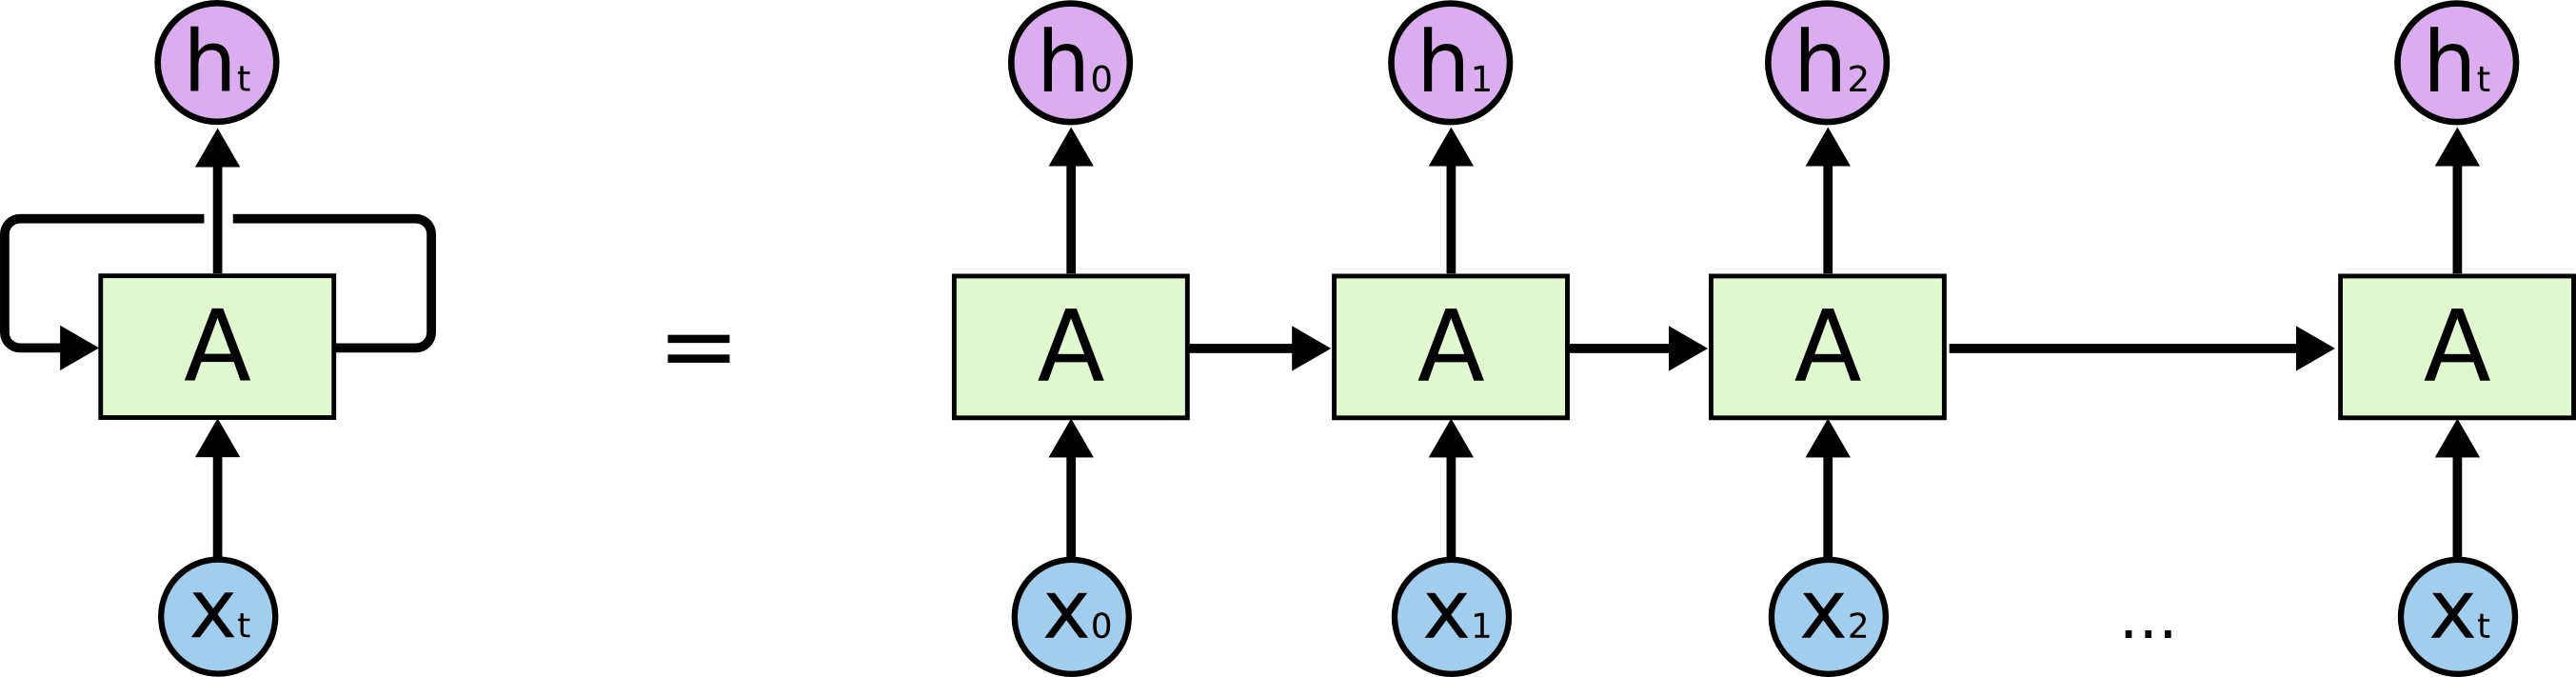
\includegraphics[width=0.75\textwidth,keepaspectratio]
		{RNN-unrolled.png}
	\end{center}
	\caption{Biểu diễn RNN theo thời gian (thứ tự trong sequence)} 
	\label{fig:pho-ofdm} 
\end{figure}
    
    Bài blog rất nổi tiếng của Andrew Karpathy đã nói về tính hiệu quả của RNN, tuy nhiên RNN có một số vấn đề, nên thực tế biến thể của nó là LSTM được sử dụng nhiều hơn.
    
    Ví dụ trong trường hợp chuỗi dữ liệu cho RNN quá dài, những dữ liệu ban đầu cũng ảnh hưởng đến đầu ra cho dù những dữ liệu ấy có thể không còn liên quan đến dữ liệu hiện tại:
    	\begin{figure} [h!]
    	\begin{center}
    		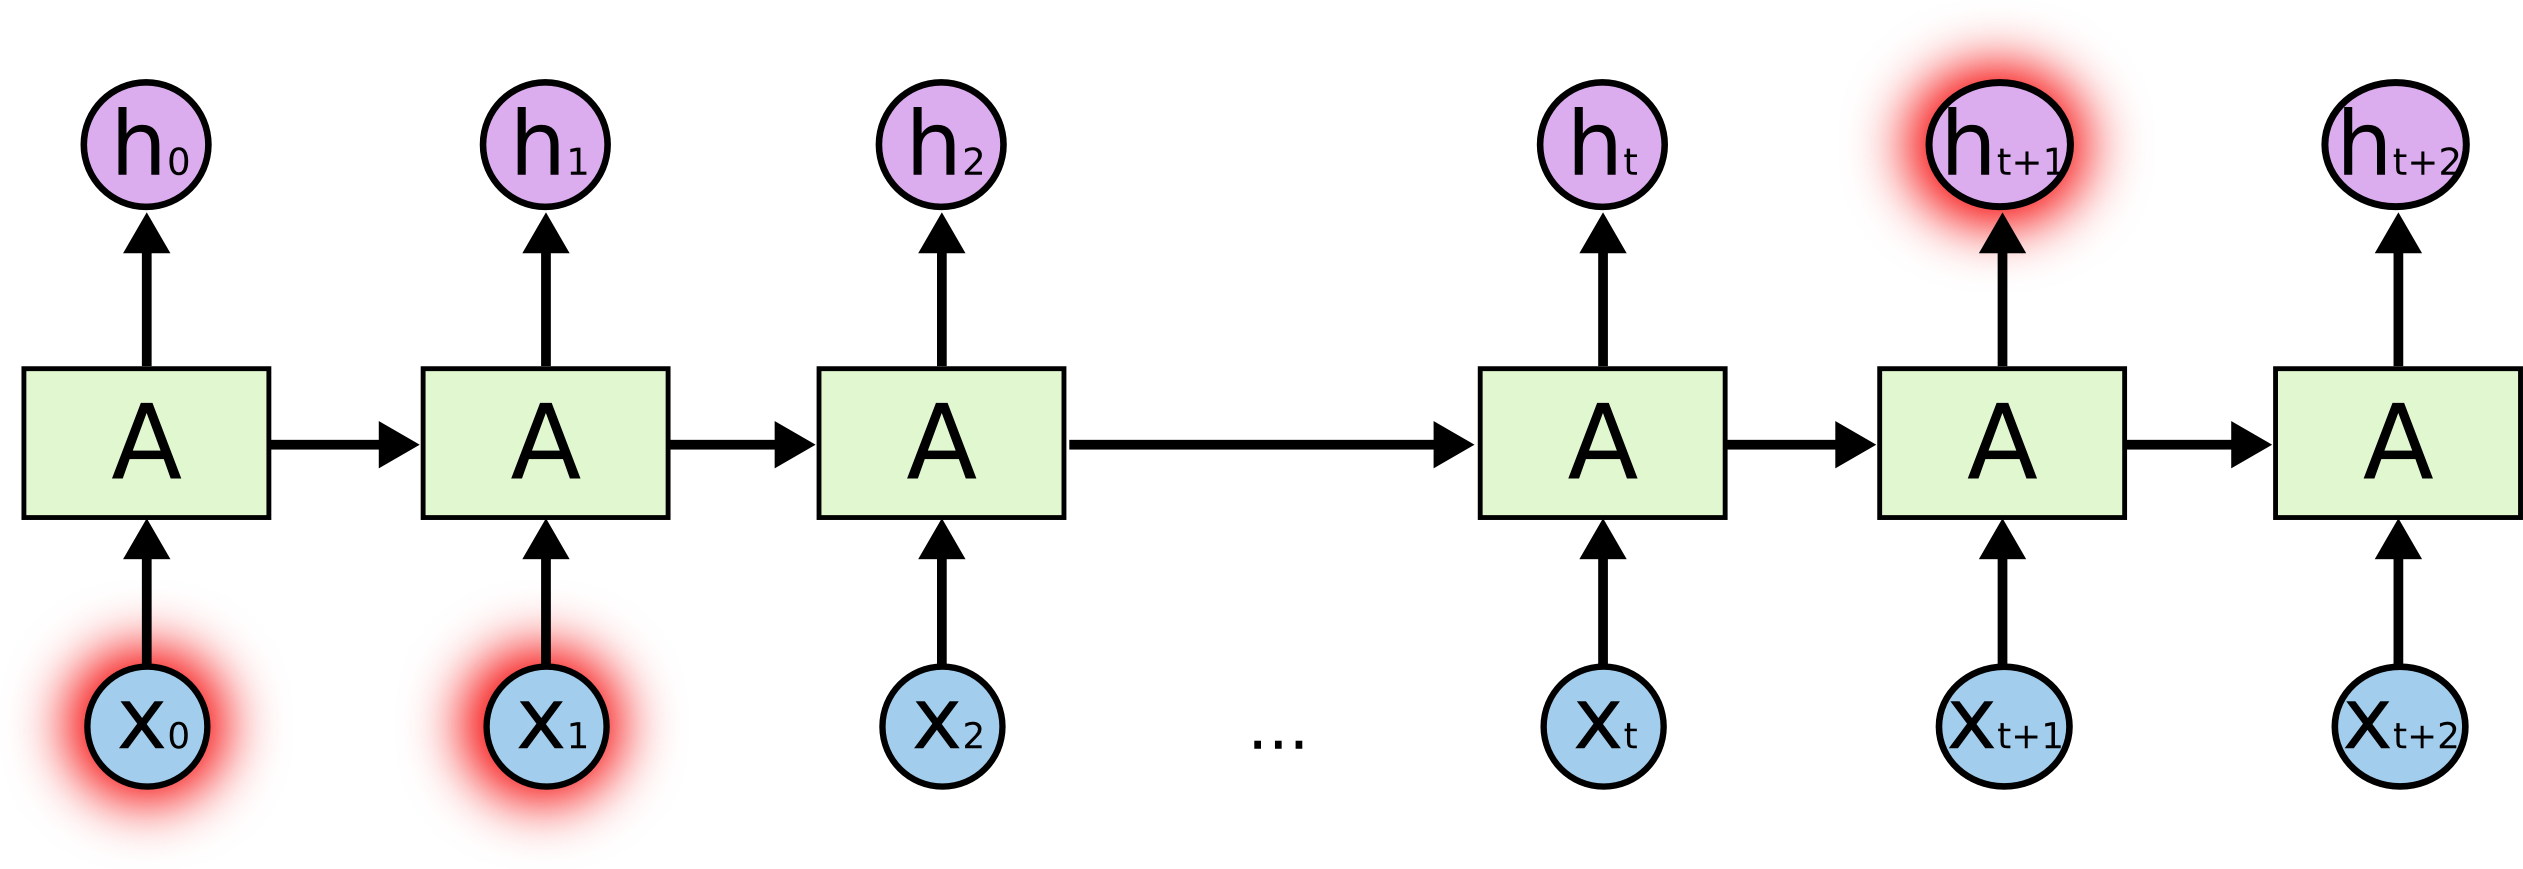
\includegraphics[width=0.75\textwidth,keepaspectratio]
    		{RNN-longtermdependencies.png}
    	\end{center}
    	\caption{Long term memory ảnh hưởng đến RNN} 
    	\label{fig:pho-ofdm} 
    \end{figure}


   Trường hợp chúng ta mong muốn đó là dữ liệu đầu vào của RNN chỉ ảnh hưởng đến đầu ra ở một thời điểm xác định như sau:
 
	\begin{figure} [h!]
	\begin{center}
		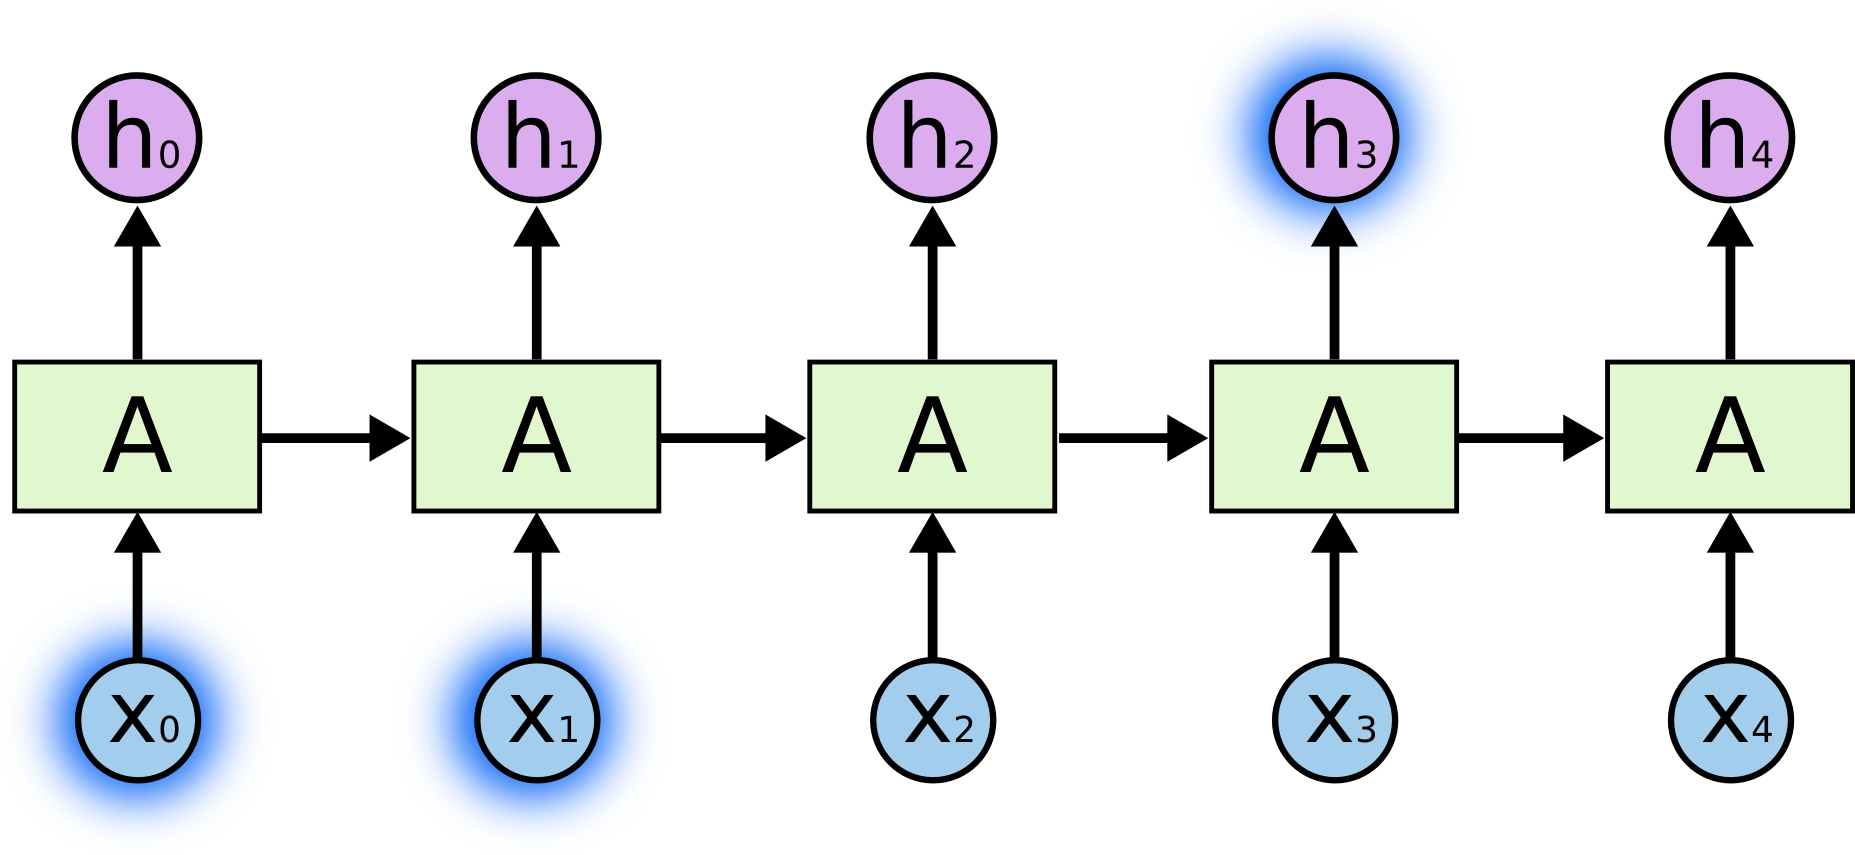
\includegraphics[width=0.75\textwidth,keepaspectratio]
		{RNN-shorttermdepdencies.png}
	\end{center}
	\caption{Biểu diễn RNN theo thời gian (thứ tự trong sequence)} 
	\label{fig:pho-ofdm} 
\end{figure}


\subsection{Long Short Term Memory}
    LSTM là một biến thể của RNN, trong đó các mạng nơ-ron không chỉ sử dụng dữ liệu từ các điểm dữ liệu trước mà còn có cổng "quên" để các giá trị quá xa trong quá khứ không ảnh hưởng đến các giá trị hiện tại.
    
    
\begin{figure} [h!]
	\begin{center}
		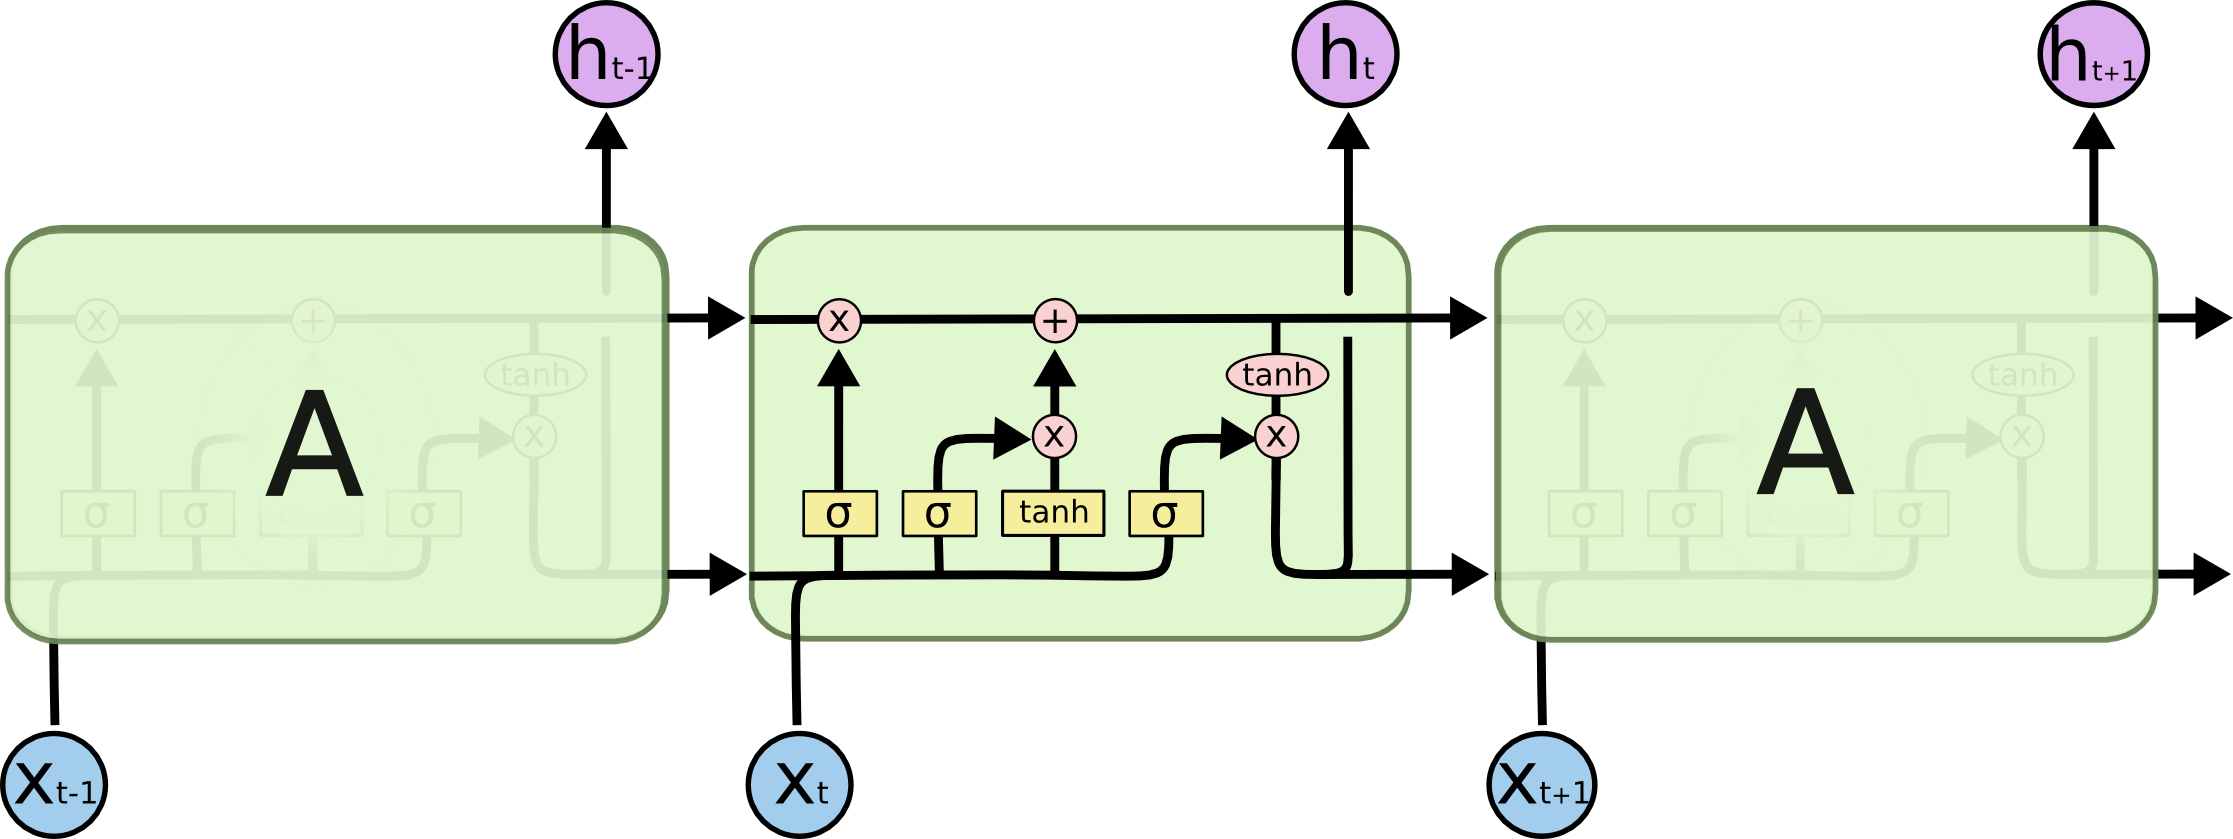
\includegraphics[width=0.75\textwidth,keepaspectratio]
		{LSTM3-chain.png}
	\end{center}
	\caption{Ví dụ 1 cell của LSTM} 
	\label{fig:pho-ofdm} 
\end{figure} 


\begin{figure} [h!]
	\begin{center}
		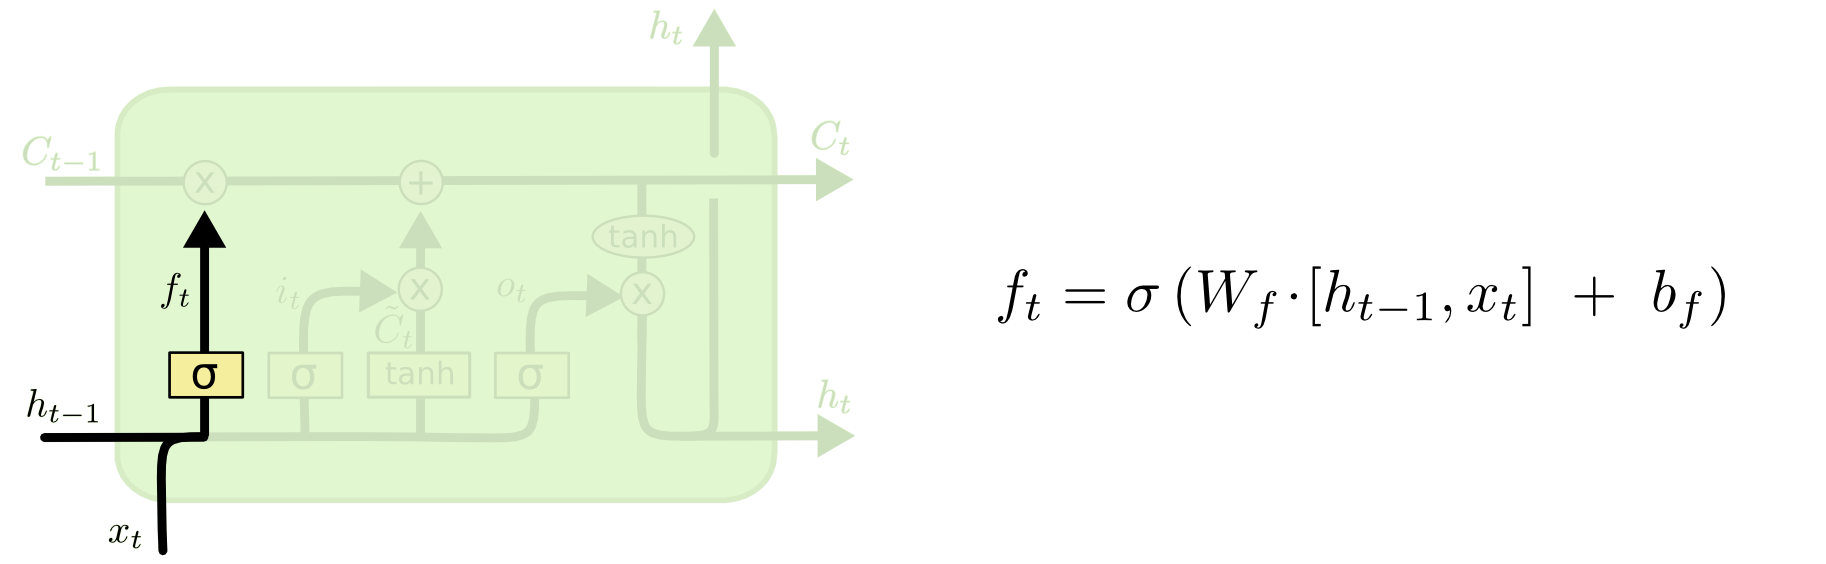
\includegraphics[width=0.75\textwidth,keepaspectratio]
		{LSTM3-focus-f.png}
	\end{center}
	\caption{Ví dụ 1 cell của LSTM} 
	\label{fig:pho-ofdm} 
\end{figure} 


    Hình dưới thể hiện cổng "quên" của 1 cell LSTM, đây là một lớp nơ-ron sigmoid có input là đầu ra của cell trước đó $\mathbf{h_{t-1}}$ và trọng số $\mathbf{W_{f}}$.
\begin{figure} [h!]
	\begin{center}
		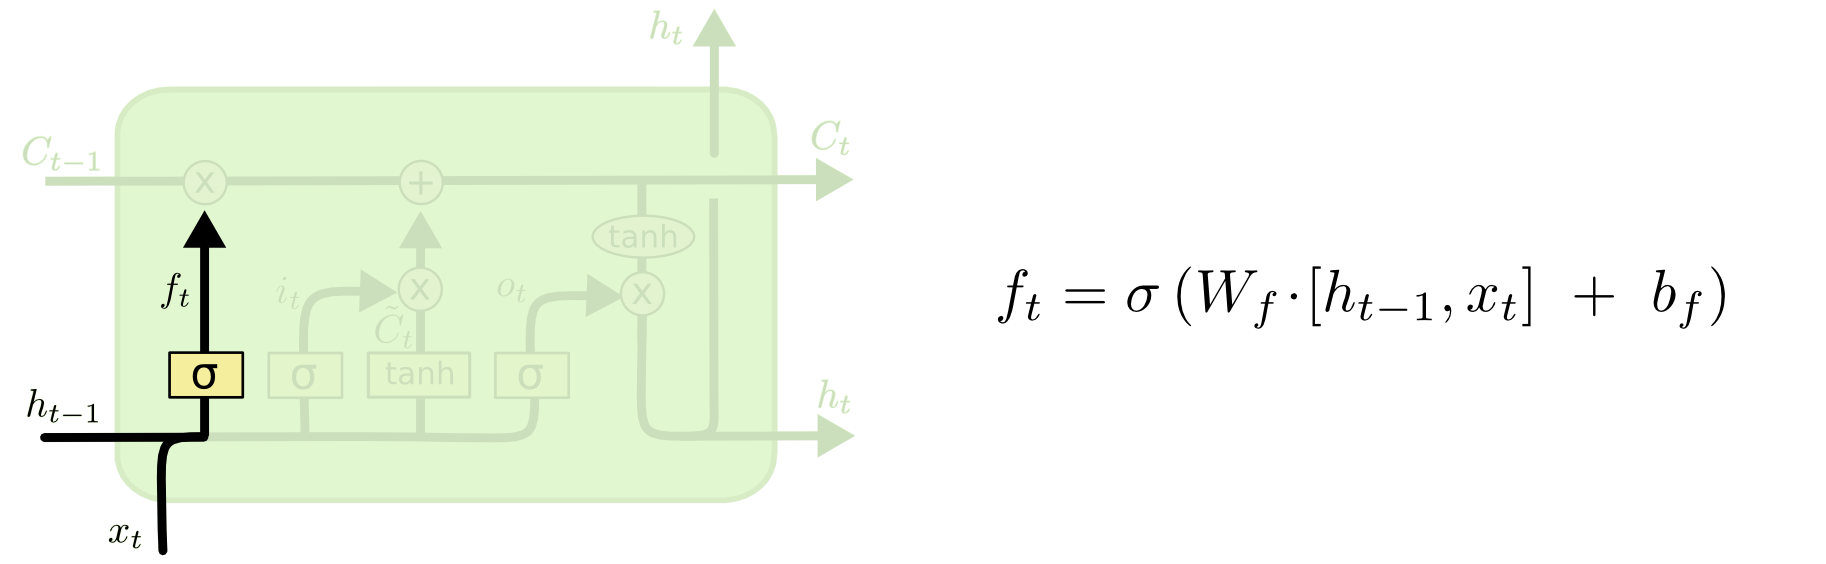
\includegraphics[width=0.75\textwidth,keepaspectratio]
		{LSTM3-focus-f.png}
	\end{center}
	\caption{Ví dụ 1 cell của LSTM} 
	\label{fig:pho-ofdm} 
\end{figure} 

    Cổng quên này có thể có giá trị giữa 0 và 1, 0 tức cell sau hoàn toàn "quên" các giá trị từ cell trước, 1 tức là cell sau nhận toàn bộ giá trị của cell trước.
    
    \begin{figure} [h!]
    	\begin{center}
    		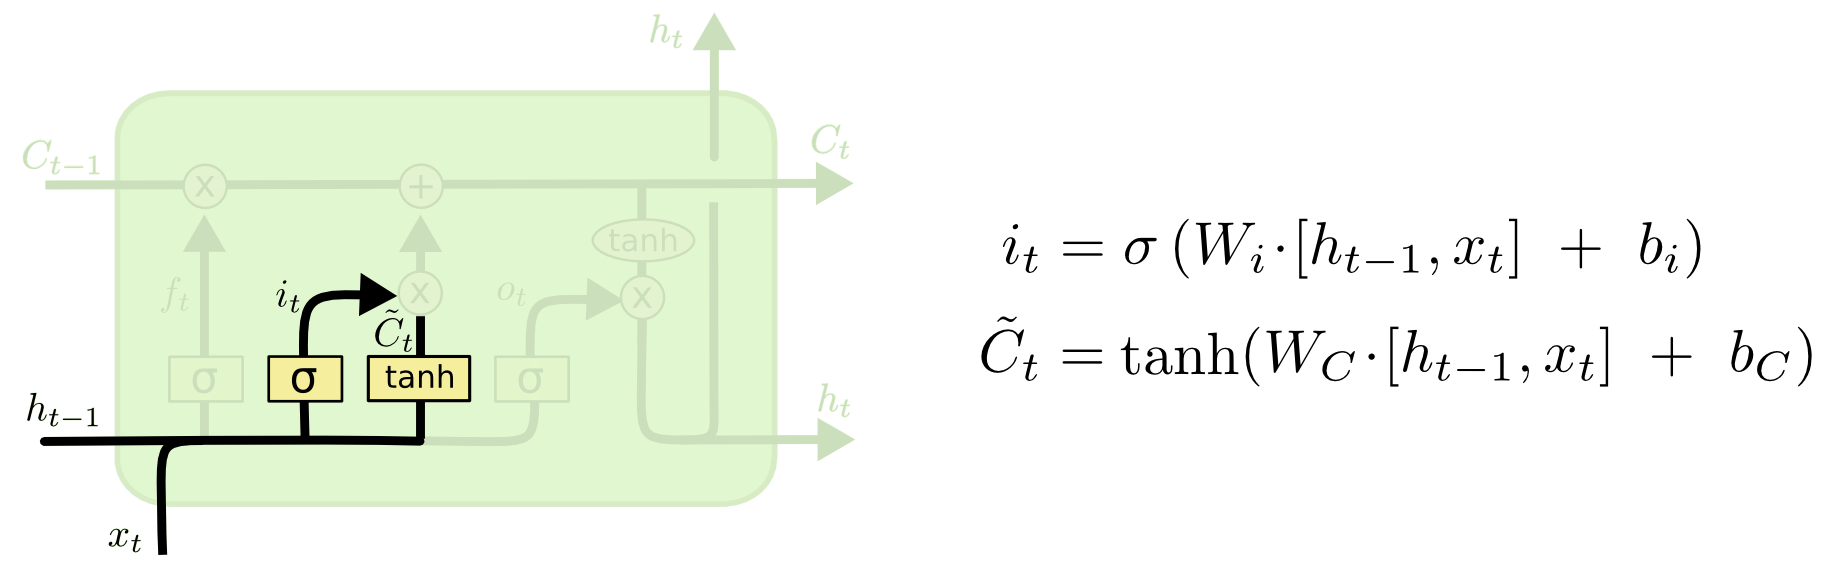
\includegraphics[width=0.75\textwidth,keepaspectratio]
    		{LSTM3-focus-i.png}
    	\end{center}
    	\caption{Ví dụ 1 cell của LSTM} 
    	\label{fig:pho-ofdm} 
    \end{figure} 
    
    Tiếp theo ta có cổng input, giá trị trạng thái tiềm năng $\mathbf{\hat{C_{t}}}$ của cell sẽ được cập nhật theo công thức như hình, giá trị này được tính bằng một lớp nơ-ron tanh với input là giá trị đầu vào $\mathbf{h_{t-1}}$  và giá trị input của cell hiện tại là $\mathbf{x_{t}}$, đầu ra của cổng này được nhân pointwise với giá trị của output cell trước với một lớp sigmoid.
    
    
\begin{figure} [h!]
	\begin{center}
		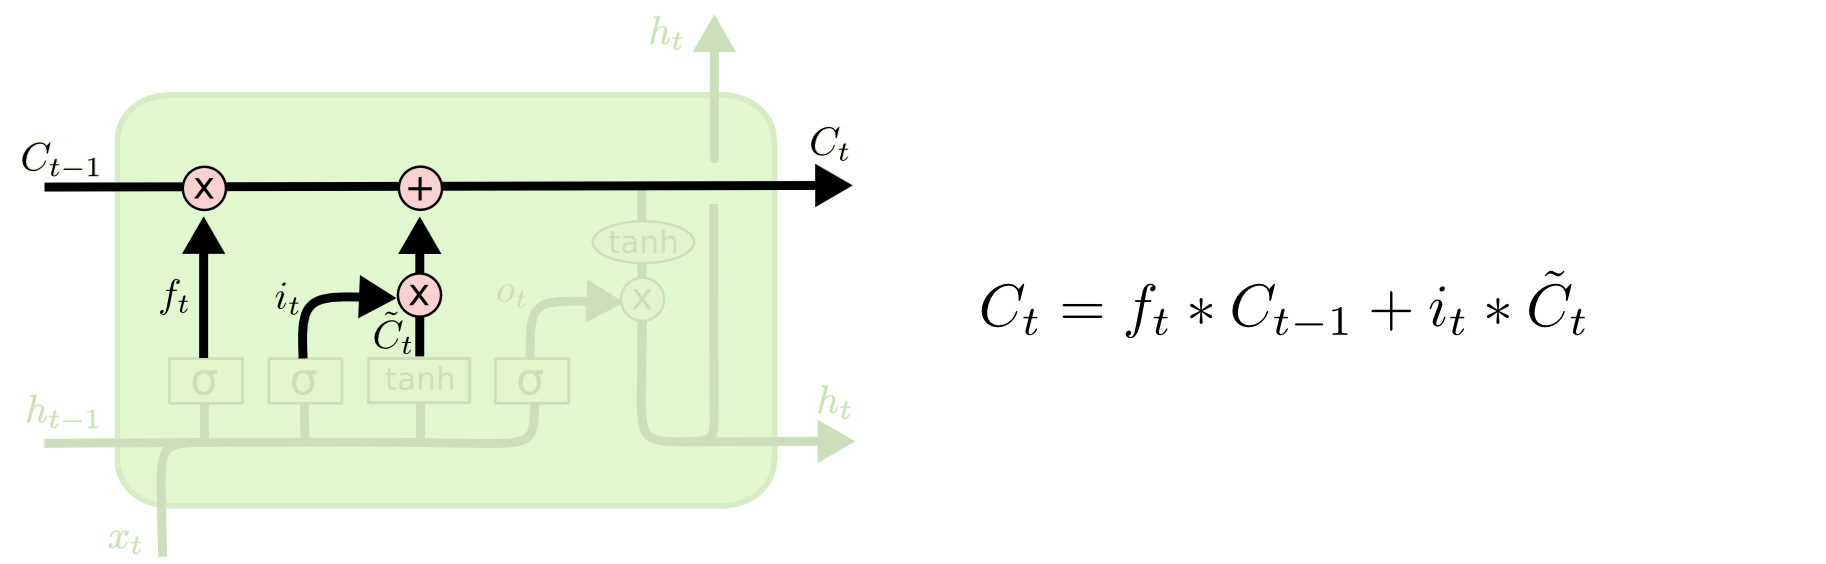
\includegraphics[width=0.75\textwidth,keepaspectratio]
		{LSTM3-focus-C.png}
	\end{center}
	\caption{Ví dụ 1 cell của LSTM} 
	\label{fig:pho-ofdm} 
\end{figure} 
    Tiếp tục với bước cập nhật giá trị $\mathbf{C_{t}}$ theo công thức như hình trên, ta nhận giá trị $\mathbf{\hat{C_{t}}}$ với giá trị quên đã tính ở trước và cộng với giá trị 


    Cuối cùng, cổng output của cell như sau:
        
    \begin{figure} [h!]
    	\begin{center}
    		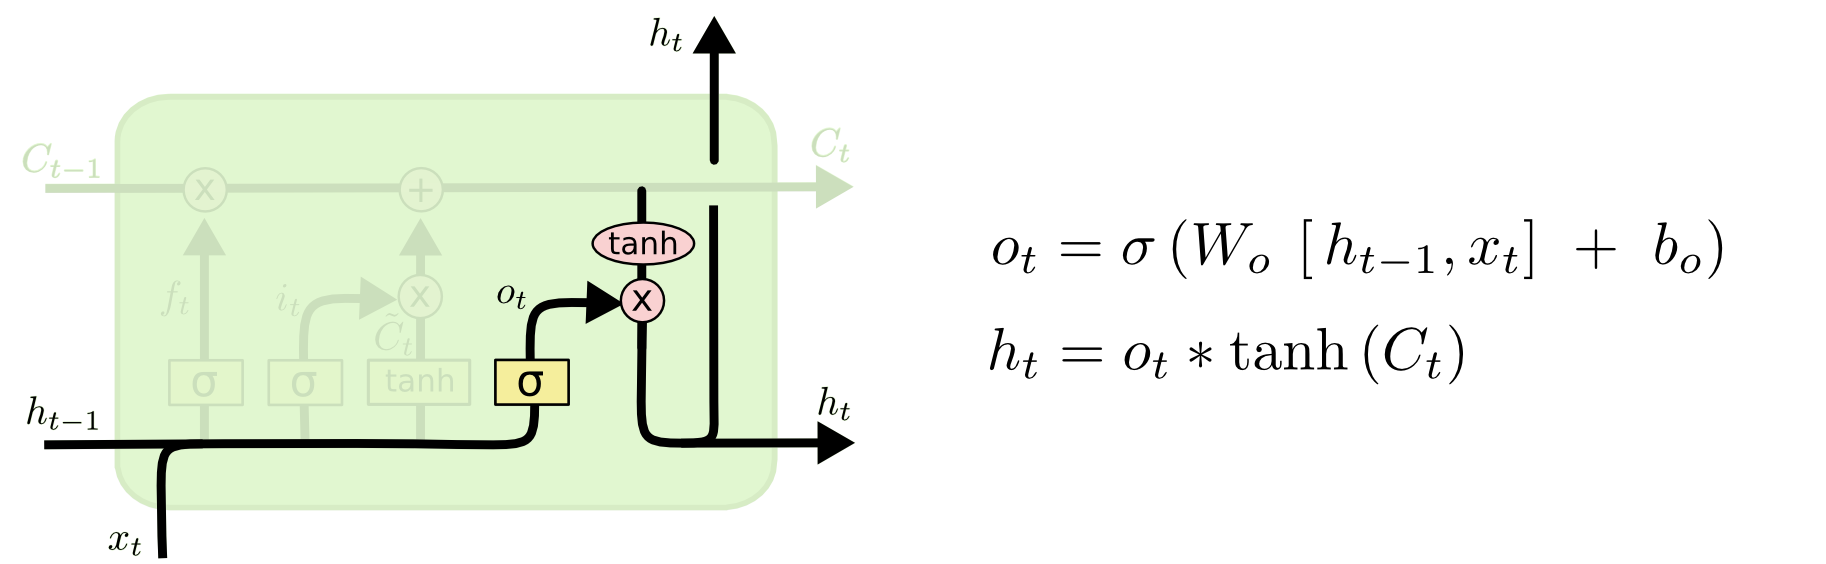
\includegraphics[width=0.75\textwidth,keepaspectratio]
    		{LSTM3-focus-o.png}
    	\end{center}
    	\caption{Ví dụ 1 cell của LSTM} 
    	\label{fig:pho-ofdm} 
    \end{figure} 
    
    Giá trị output $\mathbf{h_{t}}$ được tính dựa trên trạng thái của cell $\mathbf{C_{t}}$ sau khi qua một lớp mạng nơ-ron tanh (để đưa giá trị về đoạn - 1 đến 1), giá trị này được nhân với giá trị đầu ra của lớp trước sau khi qua một lớp sigmoid.
    
	\subsection{Cách sử dụng Latex cho báo cáo luận văn}
   
	Các sinh viên muốn đọc hiểu thêm về cách sử dụng Latex căn bản có thể tham khảo tại đây: \url{https://tobi.oetiker.ch/lshort/lshort.pdf}.
	Các sinh viên chỉ muốn hiểu đủ để viết báo cáo luận văn, có thể đọc trong báo cáo này.
	
	Việc sinh viên cần làm là viết các nội dung vào các file tương ứng trong thư mục con ``Text'' đi kèm với thư mục chính này.
	Cụ thể, sinh viên viết lời cảm ơn vào file ``loicamon.tex'', viết tóm tắt tiếng Việt vào file ``tomtatviet.tex'', viết tóm tắt tiếng Anh vào file ``tomtateng.tex'', và viết nội dung các chương vào các file tương ứng.

	Sau đó, sinh viên mở file ``thesis.tex'' trong thư mục chính.
	Trong file này, các dòng lệnh \verb|\newcommand| là định nghĩa các biến số.
	\begin{exam}
		\verb|\newcommand\studenta{Nguyễn Văn A}|: định nghĩa biến tên ``studenta'' có giá trị là ``Nguyễn Văn A''.
	\end{exam}
	Sinh viên chỉnh các biến số này cho phù hợp với họ tên, MSSV, tên luận văn, giảng viên hướng dẫn, ngày giao nhiệm vụ luận văn, ngày hoàn thành nhiệm vụ luận văn, và nội dung nhiệm vụ luận văn.
	Nếu có 2 sinh viên làm cùng một đề tài, cần tìm các dòng có biến số ``studentb'' và ``mssvb'' và bỏ dấu \% phía trước dòng tương ứng đó.
	Dấu \% nghĩa là dòng này là dòng comment, tương tự trong các ngôn ngữ lập trình.

	Sau cùng, sinh viên chạy biên dịch file ``thesis.tex'' là xong. 
	Dàn trang này đã tối ưu hóa cho việc in 2 mặt báo cáo. 
	Sinh viên chỉ cần in 2 mặt toàn bộ file ``thesis.pdf'' là có thể đóng tập hoàn chỉnh.
	
\section{Cách viết chương cơ sở lý thuyết}
	
	\subsection{Nội dung chính}
	
	Trong chương này, cơ sở lý thuyết về các vấn đề có liên quan như mô hình toán học, giải thuật, phương pháp, và các công trình đã công bố v.v. sẽ được trình bày.
	Do đó, sinh viên cần nắm cách sử dụng tài liệu tham khảo, cách viết công thức toán học, và cách trình bày hình ảnh cũng như sơ đồ.
	
	\begin{exam}
	Một luận văn làm về hệ thống truyền dẫn quang không dây dùng ánh sáng khả kiến, \ac{vlc}. Trong đó, sinh viên dùng mạng neuron tích chập, \ac{cnn}, để cân bằng miền tần số cho tín hiệu ghép kênh phân chia theo tần số trực giao, \ac{ofdm}. Các mục cần trong chương này là: 
		\begin{itemize}
			\item Sơ đồ khối và phương pháp hoạt động của \ac{vlc}, 
			\item Sơ đồ khối và giải thuật \ac{cnn}, 
			\item Khái niệm về cân bằng miền tần số, 
			\item Sơ đồ khối và phương pháp điều chế / giải điều chế \ac{ofdm},	
			\item Nội dung một số bài báo tham khảo chính để thực hiện đề tài (nếu có),
			\item Kết luận chương.
		\end{itemize}
	\end{exam}
	
	Cần lưu ý là trong báo cáo chỉ được phép có tối đa 3 mức chỉ mục, chẳng hạn có 1, 1.1, 1.1.1, nhưng không có 1.1.1.1.
	Do đó, sinh viên cần có phân bố nội dung cho phù hợp.
	Chỉ mục lớn nhất là lệnh \verb|\chapter|, chỉ mục thứ hai là lệnh \verb|\section|, và chỉ mục thứ ba là lệnh \verb|\subsection|

	Khi tạo chỉ mục, cần có ít nhất hai chỉ mục đồng cấp, chẳng hạn có 1.1.1 và 1.1.2. 
	Nếu chỉ có một chỉ mục, chẳng hạn chỉ có 1.1.1, thì không cần tạo chỉ mục.
	
	\subsection{Cách viết tắt}
	
	Nếu muốn viết tắt một cụm danh từ dài (chẳng hạn như tên một phương pháp tính toán), thì cần định nghĩa từ viết tắt ở lần đầu tiên cụm danh từ đó xuất hiện trong báo cáo.
	Những lần sau khi cụm danh từ này xuất hiện ta chỉ cần viết bằng từ viết tắt.
	Ngoài ra, danh sách từ viết tắt cần được đặt ở trước phần nội dung các chương và cần được xếp theo thứ tự chữ cái.
	
	Do đó, nếu tạo danh sách này theo cách thủ công, việc xóa hay thay đổi vị trí các đoạn văn trong quá trình chỉnh sửa có thể làm thay đổi danh sách cũng như cách viết mà không kiểm tra được.
	
	Sinh viên có thể dùng thư viện ``glossary'' của Latex để tạo danh sách từ viết tắt. 
	Tuy nhiên, thư viện này đòi hỏi cài đặt ngôn ngữ Perl.
	Bản template này dùng thư viện ``acro'', vốn không linh hoạt như thư viện ``glossary'' nhưng không đòi hỏi cài đặt thêm.
	
	Sinh viên có thể tham khảo cách định nghĩa một từ viết tắt trong file ``tuviettat.tex'' trong thư mục ``Text''.
	Trong đó, mỗi từ viết tắt có một nhãn, tên tắt và tên đầy đủ.
	Mỗi lần cần viết tắt ta dùng câu lệnh \verb|\ac{nhãn}|.
	Chẳng hạn, lệnh \verb|\ac{snr}| để viết tắt \ac{snr}.
	Chương trình tự động quyết định cách format từ viết tắt cũng như tạo danh sách đúng chuẩn.
	
	\subsection{Cách viết công thức toán học} 

	Các sinh viên thường copy công thức toán học dạng hình ảnh và dán vào file báo cáo để tiết kiệm thời gian.
	Việc này có hai bất lợi là tên biến số trong cùng một công thức nhưng copy từ hai nguồn khác nhau có thể khác nhau dẫn đến công thức không có ý nghĩa, và format font chữ của các công thức toán copy từ các nguồn khác nhau là khác nhau.
	Do đó, khi viết luận văn các sinh viên không được viết công thức toán bằng cách copy dạng hình ảnh này.
	
	Công thức toán là điểm mạnh của Latex. 
	Xem file ``chuong2.tex'' để thấy cách viết các công thức toán học sau.
	
	Ví dụ đầu tiên là các công thức giải tích mà các sinh viên làm về lớp vật lý và hệ thống analog thường gặp:
	\begin{equation}
		\oint _ {S}
		\mathbf {D} \cdot \mathrm {d} \mathbf {S} ={\int _{V}\rho \,\mathrm {d} V}.
		\label{eq:Gauss-law}
	\end{equation}	
	
	Đây là công thức định luật Gauss cho trường điện. 
	Trong lệnh này, \verb|\oint| nghĩa là tích phân (integral) toàn mặt kín.
	\verb|\_{S}| nghĩa là tên mặt kín $S$ nằm dưới dấu tích phân.
	\verb|\mathbf {D}| nghĩa là biến $\mathbf {D}$ viết đậm do là ký hiệu vector.
	\verb|\cdot| nghĩa là dấu tích vô hướng vector.
	\verb|\mathrm {d}| nghĩa là chữ d là vi phân viết thường.
	\verb|\rho| nghĩa là biến chữ cái Hy Lạp $\rho$.
	\verb|V| nghĩa là chữ $V$ viết ở dạng biến số in nghiêng.
	
	Khi viết công thức trong Latex, công thức đã được tự động đánh số theo đúng chuẩn.
	Lệnh \verb|\label{eq:ten-cong-thuc}| dùng để đặt nhãn cho công thức và tham khảo đến sau này bằng lệnh \verb|\eqref{eq:ten-cong-thuc}|.
	
	Lưu ý khi viết công thức cần giải thích rõ các biến số và đơn vị (nếu có) trong công thức.
	Chẳng hạn, trong công thức \eqref{eq:Gauss-law}, $\mathbf {D}$ (C/m$^2$) là vector mật độ điện thông đi qua mặt kín $S$ (m$^2$), và $\rho$ (C/m$^3$) là mật độ điện tích trong thể tích $V$ (m$^3$) nằm trong mặt kín $S$. 
	Khi đọc bản thảo trong file ``chuong2.tex'', sinh viên sẽ thấy các dấu ``\$'' trong câu trên nhằm viết phần nằm giữa chúng theo định dạng công thức toán học.
	Chẳng hạn viết \verb|$V^2$| sẽ là $V^2$.			
	
	Một ví dụ khác sử dụng tổng thay vì tích phân là:
	\begin{equation}
		RMSE=\frac{1}{m} \sum_{j=1}^{m} \mathbf{\left(\hat{c}-c\right)}^2. 
		\label{eq:ga_E}
	\end{equation}

	Công thức \eqref{eq:ga_E} là công thức ước lượng sai số trung bình bình phương, \ac{rmse}, giữa vector thực $\mathbf{c}$ và vector ước lượng $\mathbf{\hat{c}}$ sau $m$ lần đo đạc. 
	Đây là công thức thường gặp trong các bài toán xử lý tín hiệu.
	
	Một ví dụ dạng ma trận cho các lĩnh vực liên quan đến đại số tuyến tính là:
	\begin{equation}
		\mathbf{S} = 
			\begin{bmatrix}
				S_{11} & S_{12}\\
				S_{21} & S_{22}
				\end{bmatrix}
				=
				\begin{bmatrix}
				0.7 \angle -110^{\circ} & 0.08 \angle 60^{\circ}\\
				4 \angle 60^{\circ} & 0.6 \angle -70^{\circ}
			\end{bmatrix}.
		\label{eq:S-matrix}
	\end{equation}
	
	Trong công thức \eqref{eq:S-matrix}, ma trận $\mathbf{S}$ là ma trận tán xạ của một mạng hai cửa siêu cao tần. 
	
	Tùy vào yêu cầu của báo cáo, sinh viên có thể tự tìm các cách viết công thức khác trên mạng Internet.
	
	\subsection{Cách chèn hình vẽ} \label{sec:chen-hinh-ve}

	Trong chương \ref{sec:chuong-2}, sinh viên thường dùng các hình vẽ có sẵn với các định dạng phổ biến như .jpg và .png.
	Để chèn một hình (chẳng hạn tên là ``ofdm.png'') vào báo cáo, sinh viên copy hình tương ứng vào thư mục ``Figure'' và tham khảo đoạn code trong mục \ref{sec:chen-hinh-ve} để chèn hình ảnh.
	
	Sinh viên cần lưu ý rằng, khác với Word, Latex sẽ tự tìm vị trí tốt nhất để chèn hình ảnh này vào văn bản khi dàn trang.
	Hình ảnh có thể nằm phía trên, phía dưới, thậm chí nằm khác trang với đoạn văn miêu tả về hình ảnh.
	Do đó, tránh dùng cách miêu tả như ``trong hình dưới, ta thấy phổ của tín hiệu \ac{ofdm}'' mà phải tham chiếu đến nhãn đúng của hình bằng lệnh \verb|\ref{fig:nhãn-hình}|.
	Trong báo cáo mẫu này nhãn của hình phổ \ac{ofdm} được đặt là ``fig:pho-ofdm'' và ta có thể tham chiếu đến Hình \ref{fig:pho-ofdm} bằng lệnh \verb|\ref{fig:pho-ofdm}|.
	
	Ngoài ra, khi tham khảo trong báo cáo mẫu sinh viên sẽ thấy số 0.75 trong phần lệnh vẽ hình.
	Con số này nghĩa là scale hình lại bằng 0.75 độ rộng văn bản.
	Sinh viên có thể chỉnh số này để có hình nhỏ hoặc lớn hơn sao cho có thể xem được rõ.
	
	Trong quá trình chỉnh sửa, khi thay đổi vị trí hình, danh sách hình sẽ được cập nhật tự động.
	
	\begin{figure} [ht]
		\begin{center}
				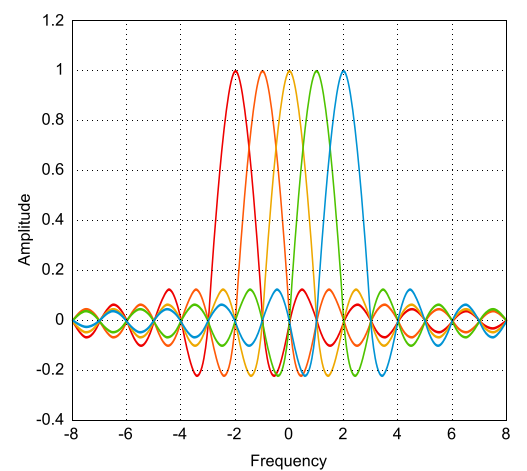
\includegraphics[width=0.75\textwidth,keepaspectratio]
				{ofdm.png}
		\end{center}
		\caption{Phổ tín hiệu \ac{ofdm}} 
		\label{fig:pho-ofdm} 
	\end{figure}
		
	\subsection{Cách thêm và sử dụng tài liệu tham khảo}

	Khi trình bày một nội dung, phương pháp, kết quả phân tích đã ghi trong một tài liệu khác, hoặc mô hình toán chứng minh trong một tài liệu khác, sinh viên bắt buộc phải dẫn nguồn tài liệu tham khảo. 
	Trong đó, quan trọng nhất đối với luận văn đại học là tham khảo cho công thức sử dụng trong báo cáo.
	Đối với các công thức kinh điển như hệ phương trình Maxwell hay giới hạn Shannon, sinh viên có thể ghi trực tiếp không cần tham khảo.
	Đối với các công thức khác, cần ghi rõ nguồn tham khảo.
	
	\begin{exam}
		Công thức tính số bit tối ưu cho mỗi sóng mang trong một hệ thống điều chế đa sóng mang là  \cite{bai-bao-ve-bit-loading}:
			\begin{equation}
			b_n= log_2 \left( 1 + \gamma {SNR}_n \right).
			\label{eq:bitloading}
			\end{equation}
		Trong đó, $b_n$ (bit) là số bit cho sóng mang thứ $n$, $\gamma$ là hệ số tối ưu không đơn vị, và ${SNR}_n$ là thông số \ac{snr} cho sóng mang thứ $n$.
	\end{exam}
	
	Mỗi tài liệu tham khảo trong danh sách phải đều phải được tham chiếu đến ít nhất một điểm trong nội dung. 
	Không được viết các tài liệu tham khảo không sử dụng trong nội dung.
	
	Ngoài ra, đối với sinh viên Điện tử - Viễn thông, tài liệu tham khảo phải viết theo chuẩn của Hội Kỹ sư Điện và Điện tử, \ac{ieee}.
	Có rất nhiều sinh viên bị mất điểm khi bảo vệ luận văn trước hội đồng vì cách trình bày tài liệu tham khảo sai.
	
	Trong mẫu báo cáo này, tất cả yêu cầu trình bày tài liệu tham khảo nói trên đã được tự động và chuẩn hóa theo \ac{ieee}.
	Syntax sử dụng theo dạng BibTex của Latex.
	Khi sinh viên cần lấy trích dẫn từ một nguồn chính thống, chẳng hạn trang web của IEEE (\url{https://ieeexplore.ieee.org/Xplore/home.jsp}), sinh viên cần làm các bước sau:
	\begin{itemize}
		\item Tìm bài báo trên trang IEEE, chẳng hạn bài báo sau: \url{https://ieeexplore.ieee.org/document/380108},
		\item Nhấn nút ``Cite this'' để trích thông tin tham khảo,
		\item Nhấn nút ``BibTex'' để copy thông tin tham khảo định dạng BibTex,
		\item Copy thông tin trên vào file ``tailieuthamkhao.bib'' trong thư mục ``Reference''.
	\end{itemize}
	
	Khi copy thông tin trên, sinh viên sẽ thấy dòng đầu tiên có dạng ``@ARTICLE\{380108,''.
	Chữ ``ARTICLE'' nghĩa là đây là một bài báo tạp chí khoa học.
	Dãy số ``380108'' chính là nhãn dùng để tham chiếu đến tài liệu này.
	Để thuận tiện, sinh viên nên sửa lại nhãn này cho có ý nghĩa hơn, chẳng hạn sửa lại thành ``@ARTICLE\{bai-bao-ve-bit-loading,''.
	Khi viết đến chỗ cần tham khảo tài liệu trong đoạn văn, sinh viên dùng lệnh \verb|\cite{nhãn-tài-liệu}|.
	Chẳng hạn, \verb|\cite{bai-bao-ve-bit-loading}| sẽ tạo ra tham chiếu đến tài liệu 
	\cite{bai-bao-ve-bit-loading}.
	
	Ở mức độ luận văn tốt nghiệp đại học, nhiều sinh viên tham khảo đến các nguồn khác như sách, luận văn khóa trước, và trang web.
	Các nguồn này thông thường không có thông tin định dạng BibTex tự động mà cần điền một cách thủ công.
	Sinh viên có thể mở file ``tailieuthamkhao.bib'' bằng một chương trình soạn văn bản bất kỳ để xem các ví dụ cách điền tài liệu tham khảo dạng sách \cite{IEEEexample:book_typical}, luận văn \cite{IEEEexample:masterstype}, và trang web \cite{IEEEexample:IEEEwebsite}.
	
\section{Kết luận chương}

	Phần này đưa ra tổng kết chung về chương. 
	Nếu luận văn hướng đến việc ứng dụng và so sánh các phương pháp, cần nêu điểm mạnh và điểm yếu của từng phương pháp. 
	Từ đó, giải thích được tại sao luận văn chọn phương pháp A hoặc B để trả lời câu hỏi nghiên cứu.
	
	\begin{exam}
	Trong chương này, cơ sở lý thuyết về \ac{vlc}, \ac{ofdm}, và \ac{cnn} đã được tổng kết và giới thiệu.
	Các lý thuyết này được ứng dụng phương pháp nghiên cứu được trình bày trong chương tiếp theo.
	\end{exam}